\subsection{End-to-End Platform Architecture}
\label{sec:method_overview}

\textcolor{blue}{EABench is organized as a single experimental pipeline rather than a loose collection of scripts. A scenario specification begins with a \texttt{StoryConfig}, which defines the company profile, timeline, employee count, and key events that drive narrative evolution. The tenant generator expands this specification into a multi-modal enterprise corpus containing users, emails, chats, meetings, and files. The same tenant is then consumed by the agent runtime, which executes under a concrete user identity and records its full tool trajectory. Finally, the evaluation harness scores the resulting answer with both deterministic and judge-based metrics. Because each stage writes explicit artifacts to disk, the entire process is reproducible and inspectable.}

\begin{figure}[h]
\centering
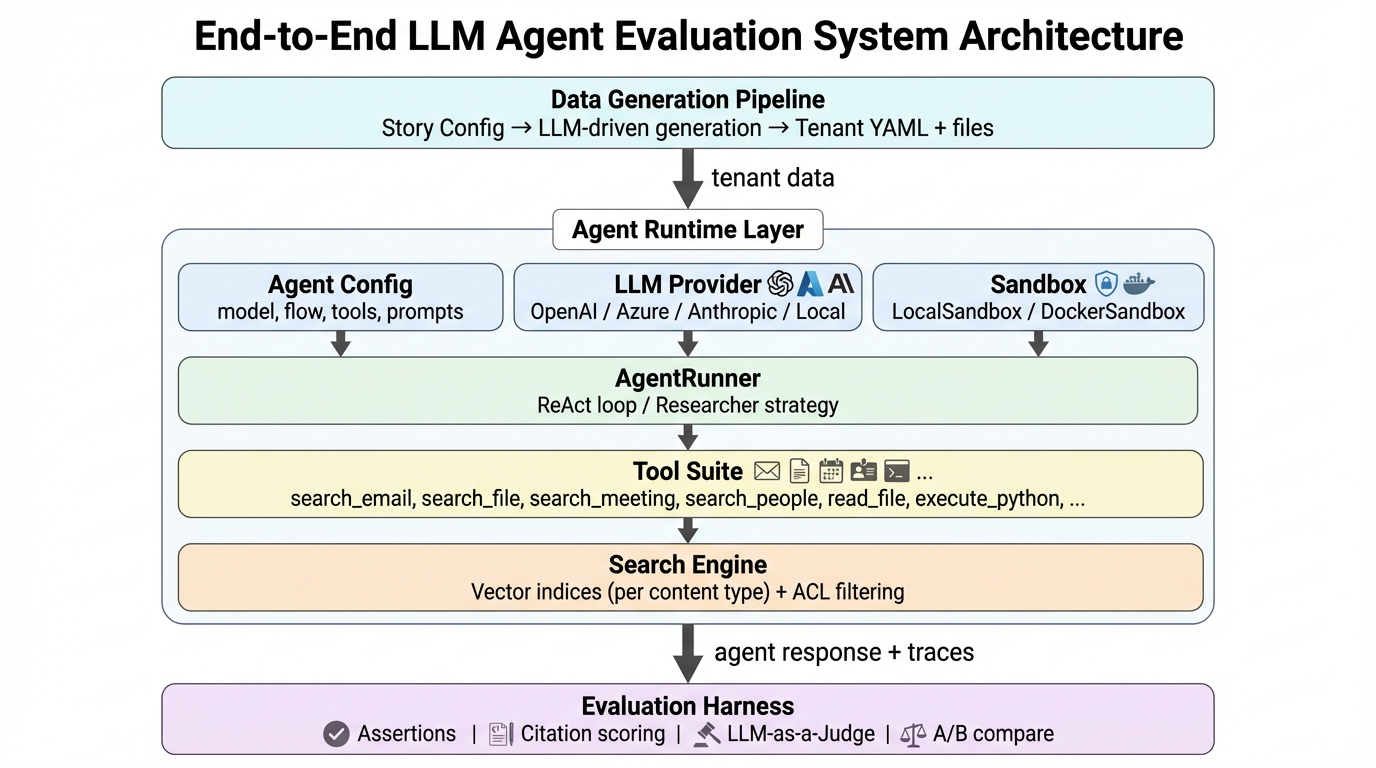
\includegraphics[width=0.85\textwidth]{figures/agent-evaluator-framework.png}
%\resizebox{0.96\linewidth}{!}{\begin{tikzpicture}[
  font=\small,
  box/.style={draw, rounded corners=2pt, align=center, minimum height=8mm},
  outer/.style={draw, rounded corners=2pt, inner sep=7pt},
  arr/.style={-{Latex[length=2mm]}, thick}
]
  % Top pipeline
  \node[box, fill=cyan!8, minimum width=0.94\textwidth] (datagen) {
    \textbf{Data Generation Pipeline}\\
    Story Config $\rightarrow$ LLM-driven generation $\rightarrow$ Tenant YAML + files
  };

  % Runtime top row (symmetric around center)
  \node[box, fill=blue!5, minimum width=0.20\textwidth, below=12mm of datagen] (llmprov) {
    \textbf{LLM Provider}\\
    OpenAI / Azure / Anthropic / Local
  };
  \node[box, fill=blue!5, minimum width=0.20\textwidth, left=12mm of llmprov] (agentcfg) {
    \textbf{Agent Config}\\
    model, flow, tools, prompts
  };
  \node[box, fill=blue!5, minimum width=0.20\textwidth, right=12mm of llmprov] (sandbox) {
    \textbf{Sandbox}\\
    LocalSandbox / DockerSandbox
  };

  % Runtime stack
  \node[box, fill=green!6, minimum width=0.68\textwidth, below=8mm of llmprov] (runner) {
    \textbf{AgentRunner}\\
    ReAct loop / Researcher strategy
  };

  \node[box, fill=yellow!10, minimum width=0.68\textwidth, below=8mm of runner] (tools) {
    \textbf{Tool Suite}\\
    search\_email, search\_file, search\_meeting, search\_people, read\_file, execute\_python, ...
  };

  \node[box, fill=orange!10, minimum width=0.68\textwidth, below=8mm of tools] (search) {
    \textbf{Search Engine}\\
    Vector indices (per content type) + ACL filtering
  };

  % Runtime container and title
  \node[outer, fit=(agentcfg)(llmprov)(sandbox)(runner)(tools)(search)] (runtime) {};
  \node[anchor=north west, fill=white, inner sep=1.2pt, font=\bfseries\small]
    at ([xshift=2mm,yshift=0.8mm]runtime.north west) {Agent Runtime Layer};

  % Bottom evaluation
  \node[box, fill=purple!8, minimum width=0.94\textwidth, below=7mm of runtime] (eval) {
    \textbf{Evaluation Harness}\\
    Assertions $\mid$ Citation scoring $\mid$ LLM-as-a-Judge $\mid$ A/B compare
  };

  % Orthogonal flows
  \draw[arr] (datagen.south) -- node[right]{\small tenant data} (datagen.south |- runtime.north);
  \draw[arr] (agentcfg.south) -- (agentcfg.south |- runner.north);
  \draw[arr] (llmprov.south) -- (runner.north);
  \draw[arr] (sandbox.south) -- (sandbox.south |- runner.north);
  \draw[arr] (runner.south) -- (tools.north);
  \draw[arr] (tools.south) -- (search.north);
  \draw[arr] (runtime.south) -- node[right]{\small agent response + traces} (runtime.south |- eval.north);
\end{tikzpicture}
}
\caption{\textcolor{blue}{End-to-end EABench architecture. The platform connects scenario specification, tenant generation, configurable runtime execution, evaluation-case generation, and interactive debugging in one reproducible workflow.}}
\label{fig:arch}
\end{figure}

\textcolor{blue}{This architecture supports two complementary use modes. In batch mode, researchers generate a tenant, evaluate one or more agent configurations, and compare the resulting metric distributions. In interactive mode, they run the same runtime against the same tenant but inspect intermediate search results, tool calls, citations, and user context while debugging failure cases. The shared backend is important: debugging traces come from the exact runtime that produces benchmark results, so qualitative inspection and quantitative evaluation remain aligned.}

\begin{table}[h]
\centering
\caption{\textcolor{blue}{Primary artifacts exchanged across the EABench pipeline.}}
\label{tab:pipeline_artifacts}
\small
{\color{blue}
\begin{tabular}{p{0.17\linewidth}p{0.24\linewidth}p{0.48\linewidth}}
\toprule
\textbf{Stage} & \textbf{Primary artifact} & \textbf{Role in the pipeline} \\
\midrule
Scenario specification & \texttt{StoryConfig} and prompt templates & Defines the enterprise domain, timeline, narrative drivers, and generator behavior \\
Tenant generation & \texttt{tenant.yaml}, \texttt{generation\_log.json}, modality-specific YAML files, sandbox files & Materializes a coherent enterprise workspace with explicit provenance \\
Evaluation dataset generation & \texttt{eval\_dataset\_*.yaml} & Converts raw tenant history into query cases with \texttt{user\_id}, \texttt{entity\_list}, and weighted assertions \\
Agent runtime & Response text, tool traces, token and latency metrics & Executes a concrete agent configuration under a specific access context \\
Evaluation harness & Per-case JSON results and aggregate summaries & Produces assertion, citation, and operational diagnostics for comparison and analysis \\
Interactive debugging & Search evidence, tool-call logs, citation traces & Explains success and failure modes on individual cases without changing the runtime \\
\bottomrule
\end{tabular}
}
\end{table}

\textcolor{blue}{The key systems claim of EABench is therefore not only that each subsystem is configurable, but that the interfaces between subsystems are stable and explicit. A change in the generator alters the tenant and the resulting query set; a change in the runtime alters the trajectory and answer; a change in the judge alters the scoring layer. By exposing these seams directly, EABench makes causal experimentation possible.}